\documentclass[tikz, border=10pt]{standalone}

\usepackage{amsmath, amsfonts, mathtools, amssymb}
\usepackage{tikz}
\usetikzlibrary{calc}

\begin{document}
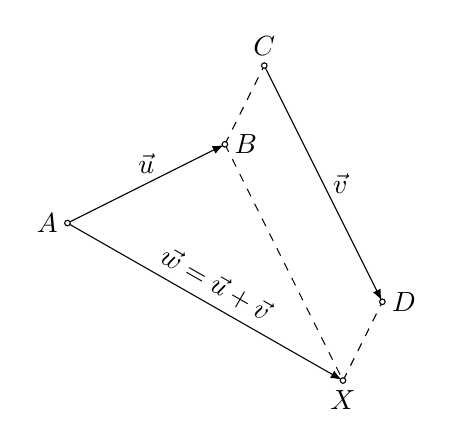
\begin{tikzpicture}
    \coordinate[label=left:$A$] (A) at (-1, 0);
    \coordinate[label=right:$B$] (B) at (1, 1);
    \coordinate[label=above:$C$] (C) at (1.5, 2);
    \coordinate[label=right:$D$] (D) at (3, -1);
    \coordinate[label=below:$X$] (X) at ($(D) + (B) - (C)$);
    \draw[-latex, shorten >=0.5pt] (A) -- (B) node[above, midway] {$\Vec{u}$};
    \draw[-latex, shorten >=0.5pt] (C) -- (D) node[right, midway] {$\Vec{v}$};
    \draw[-latex, shorten >=0.5pt] (A) -- (X) node[sloped, midway, above] {$\Vec{w} = \Vec{u} + \Vec{v}$};
    \draw[dashed] (B) -- (C) (B) -- (X) (X) -- (D);
    \foreach \point in {A, B, C, D, X}
        \path[draw, fill=white] (\point) circle (1pt);
\end{tikzpicture}
\end{document}